\chapter{حفظ الكتلة والمعادلات الموزونة}\label{ch:g8:balanced-equations}

حطبة كتلتها كيلوغرامان تحترق في الموقد. وفي الصباح تبقى بضع عشرات من
الغرامات من الرماد الرمادي. فهل تلاشى نحو كيلوغرامين من المادة في
الليل؟ ظل السؤال قرونًا بلا جواب. وجاء الجواب من كيميائي قرر أن يزن كل
شيء --- حتى الغازات التي لم يفكر أحد في وزنها.

\begin{recall}
في \omterm{def:g7:chemical-reactions:reaction}{التفاعل الكيميائي} تُستهلك \omterm{def:g7:chemical-reactions:reactant}{المتفاعلات} وتتكوّن \omterm{def:g7:chemical-reactions:reactant}{النواتج}؛ ويُعاد ترتيب \omterm{def:g7:atoms-and-molecules:atom}{ذرات}
\omterm{def:g7:chemical-reactions:reactant}{المتفاعلات} في \omterm{def:g7:chemical-reactions:reactant}{النواتج}، فلا تُخلق ولا تفنى
(\cref{ch:g7:chemical-reactions}). \omterm{def:g7:atoms-and-molecules:formula}{والصيغة الكيميائية} مثل \ce{H2O} تذكر
\omterm{def:g7:atoms-and-molecules:atom}{ذرات} \omterm{def:g7:atoms-and-molecules:molecule}{الجزيء}؛ والعدد المكتوب أمامها، كما في \ce{3H2O}، يعدّ \omterm{def:g7:atoms-and-molecules:molecule}{الجزيئات}
(\cref{ch:g7:atoms-and-molecules}).
\end{recall}

\begin{omfigure}
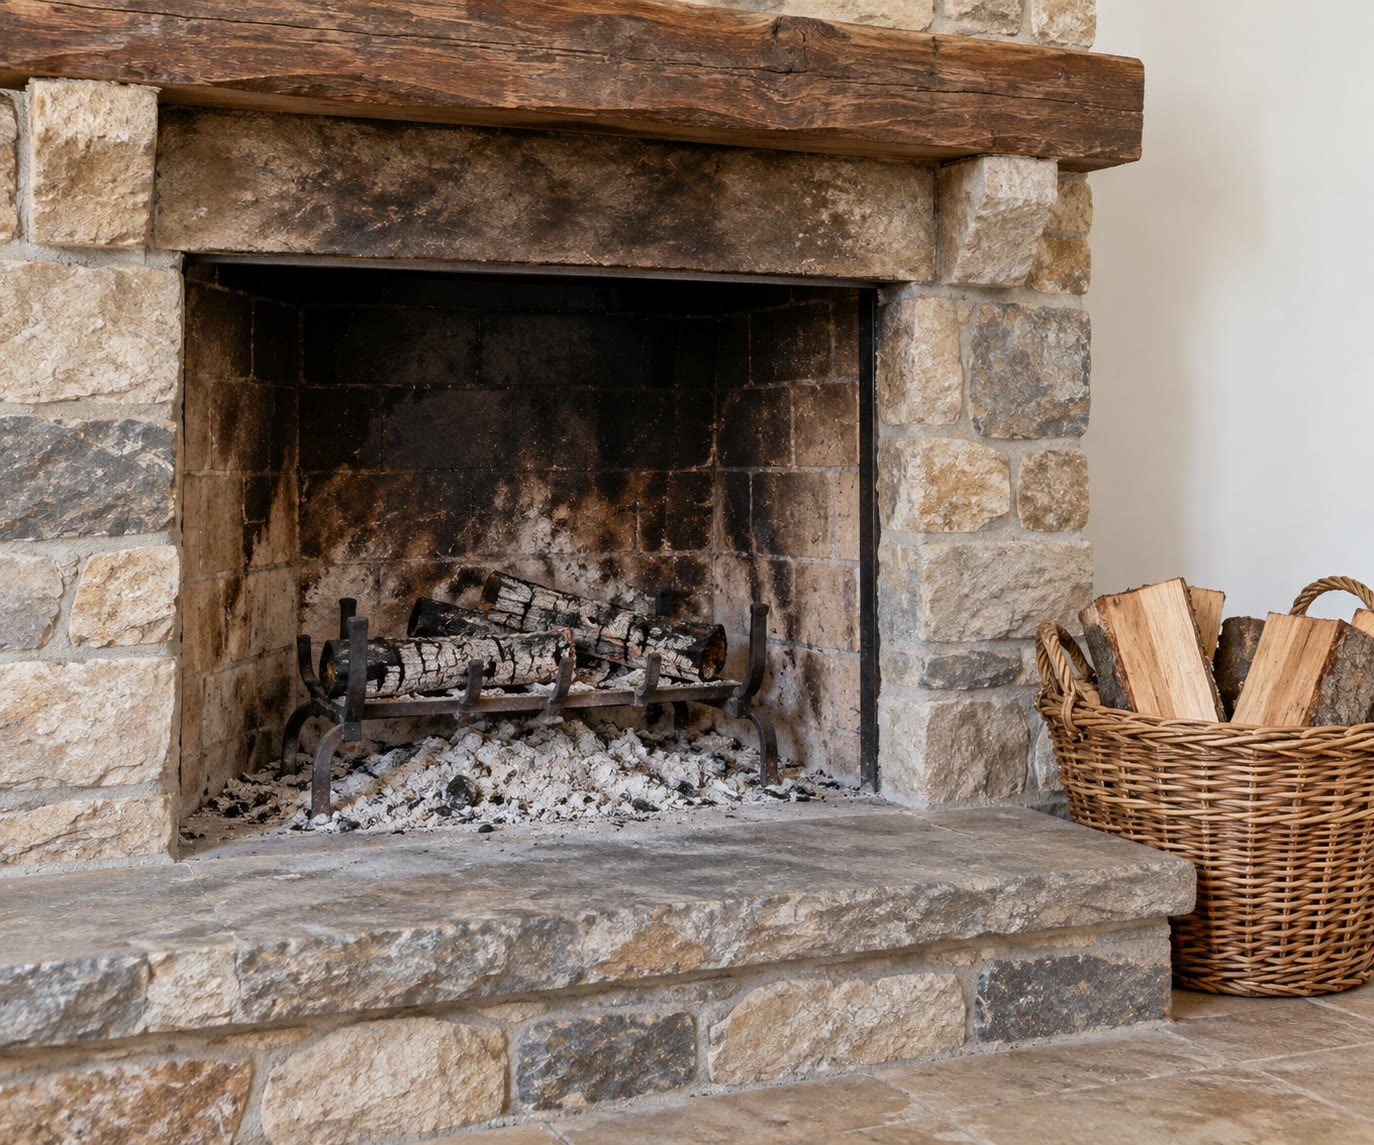
\includegraphics[width=0.5\linewidth]{images/book1/ai/g8-fireplace-ash.jpg}

{\small موقد في صباح اليوم التالي: قليل من الرماد هو كل ما بقي من
الحطب.}
\end{omfigure}

\section{الكتلة محفوظة}

\begin{inthelab}[وزن تفاعل في دورق مغلق]
يضع المعلم قليلًا من الخل في دورق، وصودا الخبز في بالون مثبت على عنقه،
ثم يضع المجموعة كلها على ميزان: \qty{212.4}{g}. يُرفع البالون فتسقط
الصودا في الخل: يفور \omterm{def:g6:pure-substances-and-mixtures:mixture}{الخليط} وينتفخ البالون بالغاز المتكوّن. ويبقى الميزان
يشير إلى \qty{212.4}{g}. أما التفاعل نفسه في دورق مفتوح، بلا بالون،
فإنه «يفقد» من الكتلة: إذ يفلت الغاز إلى الغرفة.
\end{inthelab}

\begin{omfigure}
\begin{tikzpicture}[font=\small, scale=1.15]
  % closed flask
  \pic[transform shape] at (0,0) {balance};
  \pic[transform shape] at (0,0.8) {erlenmeyer={0.25}{omWater!80}};
  \fill[red!55, draw=red!60!black] (0,4.05) ellipse (0.5 and 0.62);
  \fill[red!55] (-0.3,3.45) rectangle (0.3,3.6);
  \node[anchor=north, align=center] at (0,-0.1) {مغلق: يبقى الغاز\\ في البالون};
  \node[anchor=west, font=\footnotesize] at (1.25,0.3) {\qty{212.4}{g}};
  % open flask
  \pic[transform shape] at (4,0) {balance};
  \pic[transform shape] at (4,0.8) {erlenmeyer={0.25}{omWater!80}};
  \foreach \y in {3.6,3.95,4.3} \draw[->, black!45, decorate,
    decoration={snake, amplitude=0.6pt, segment length=4pt}] (4,\y) -- (4,\y+0.3);
  \node[anchor=north, align=center] at (4,-0.1) {مفتوح: يفلت الغاز،\\ وتنخفض القراءة};
  \node[anchor=west, font=\footnotesize] at (5.25,0.3) {\qty{211.9}{g}};
\end{tikzpicture}

{\small التفاعل نفسه، موزونًا. في الدورق المغلق لا تتغير الكتلة؛ وفي
الدورق المفتوح يخرج الغاز فيشير الميزان إلى
أقل.}
\end{omfigure}

\begin{definition}[حفظ الكتلة]\label{def:g8:balanced-equations:conservation}
\emph{حفظ الكتلة}\index{حفظ الكتلة} هو القانون الذي ينص على أنه في \omterm{def:g7:chemical-reactions:reaction}{التفاعل
الكيميائي} تساوي الكتلة الكلية للنواتج المتكوّنة الكتلة الكلية للمتفاعلات
المستهلكة. فلا يضيع شيء ولا يُخلق شيء؛ وإنما تغيّر المادة
شكلها.
\end{definition}

\begin{example}[الحطبة، موزونة كما ينبغي]\label{ex:g8:balanced-equations:log}
لو أمكن أن نزن الحطبة المحترقة والأكسجين الذي أخذته من \omterm{def:g4:air-a-mixture-of-gases:air}{الهواء} قبل
\omterm{def:g4:what-a-fire-needs:burning}{الاحتراق}، ثم الرماد وثنائي أكسيد الكربون وبخار الماء بعده، لتساوى
المجموعان. والرماد خفيف لأن معظم \omterm{def:g7:chemical-reactions:reactant}{النواتج} غازات تصعد في المدخنة.
\end{example}

\begin{history}[لافوازييه يزن كل شيء، من سبعينيات القرن الثامن عشر إلى 1789]
جعل أنطوان لوران لافوازييه من قواعده أن يزن كل مادة قبل كل تفاعل
وبعده، في أوعية محكمة الإغلاق حتى لا يفلت غاز ولا يدخل. وبيّن أن
الفلزات تكتسب كتلة حين تصدأ أو تحترق، إذ تأخذ شيئًا من \omterm{def:g4:air-a-mixture-of-gases:air}{الهواء} ---
الأكسجين، الذي سمّاه هو --- وأعلن سنة 1789 أنه لا يُخلق شيء ولا يضيع
شيء في التفاعل. وكانت زوجته، ماري آن بولز لافوازييه، تعمل إلى جانبه،
فتسجل التجارب وترسم الأجهزة لكتابه.
\end{history}

\begin{omfigure}
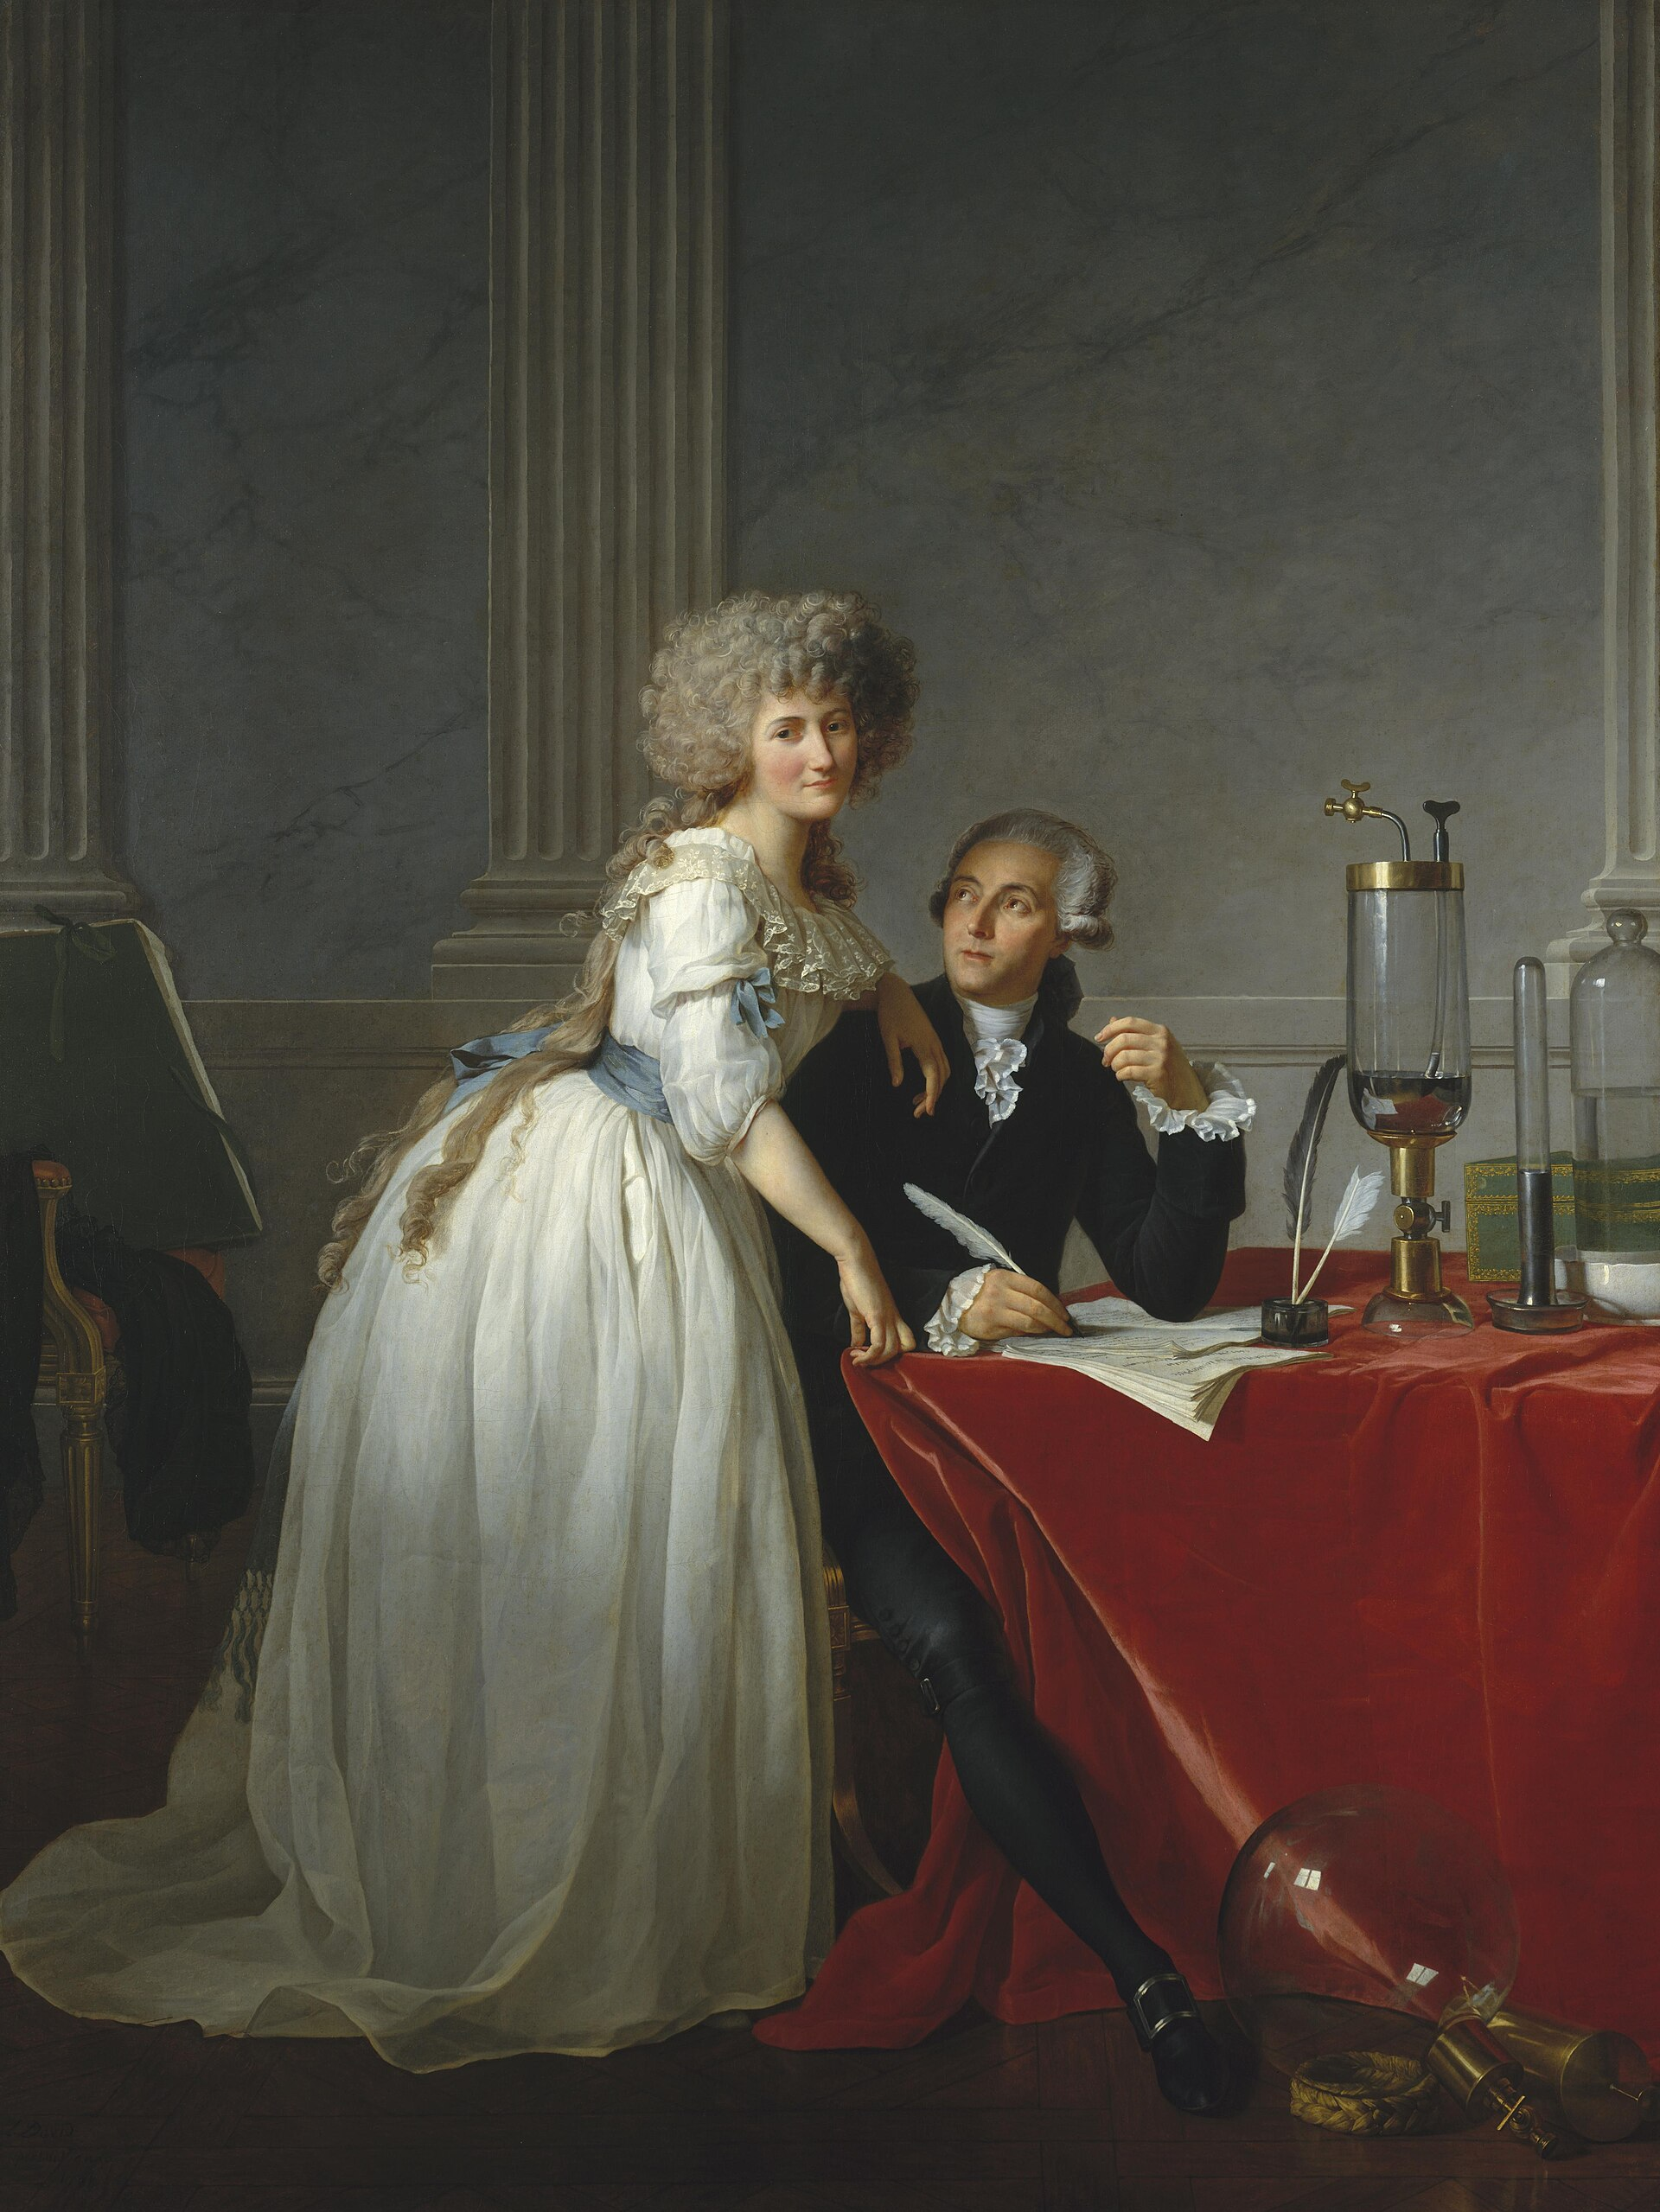
\includegraphics[width=0.3\linewidth]{images/book1/lavoisier.jpg}

{\small أنطوان لوران لافوازييه وماري آن بولز لافوازييه، بريشة
جاك لوي دافيد، 1788.}
\end{omfigure}

\section{لماذا تُحفظ الكتلة}

\begin{proposition}[الذرات محفوظة، إذن الكتلة محفوظة]\label{prop:g8:balanced-equations:why}
في التفاعل لا يحدث \omterm{def:g7:atoms-and-molecules:atom}{للذرات} إلا إعادة ترتيب: فكل \omterm{def:g7:atoms-and-molecules:atom}{ذرة} من \omterm{def:g7:atoms-and-molecules:atom}{ذرات} \omterm{def:g7:chemical-reactions:reactant}{المتفاعلات}
نجدها من جديد في \omterm{def:g7:chemical-reactions:reactant}{النواتج}. وكل \omterm{def:g7:atoms-and-molecules:atom}{ذرة} تحتفظ بكتلتها. ولذلك لا يمكن أن تتغير
الكتلة الكلية.
\end{proposition}

\begin{example}[حديد يكتسب كتلة]\label{ex:g8:balanced-equations:iron}
الصوف الفولاذي الذي يُحرق على ميزان في صحن مفتوح يزداد ثقلًا: \omterm{def:g7:atoms-and-molecules:atom}{فذرات} الحديد
اتحدت \omterm{def:g7:atoms-and-molecules:atom}{بذرات} أكسجين أُخذت من \omterm{def:g4:air-a-mixture-of-gases:air}{الهواء}، وأكسيد الحديد المتكوّن يزن الحديد
مضافًا إليه ذلك الأكسجين. أما إذا أُحرق في مخبار مغلق من \omterm{def:g4:air-a-mixture-of-gases:air}{الهواء} فوق الميزان
فإن كتلة المجموعة لا تتغير: فالأكسجين كان أصلًا داخل
المخبار.
\end{example}

\section{المعادلة الكيميائية}

\begin{definition}[المعادلة الكيميائية]\label{def:g8:balanced-equations:equation}
\emph{المعادلة الكيميائية}\index{معادلة كيميائية} تكتب التفاعل بالصيغ:
صيغ \omterm{def:g7:chemical-reactions:reactant}{المتفاعلات} على اليسار يربط بينها $+$، ثم سهم، ثم صيغ \omterm{def:g7:chemical-reactions:reactant}{النواتج} على
اليمين. وقد يُكتب أمام كل صيغة عدد. وتكون المعادلة
\emph{معادلة موزونة}\index{معادلة موزونة} إذا ظهر كل نوع من \omterm{def:g7:atoms-and-molecules:atom}{الذرات} العدد
نفسه من المرات في الطرفين.
\end{definition}

\begin{definition}[المعامل الستوكيومتري]\label{def:g8:balanced-equations:coefficient}
العدد المكتوب أمام صيغة في معادلة هو
\emph{معاملها الستوكيومتري}\index{معامل ستوكيومتري}: وهو يعدّ \omterm{def:g7:atoms-and-molecules:molecule}{الجزيئات} (أو
الجسيمات الأخرى) من ذلك النوع المشاركة في التفاعل. والمعامل 1 لا
يُكتب.
\end{definition}

\begin{notation}[رموز الحالة]\label{not:g8:balanced-equations:states}
قد يبيّن حرف بين قوسين بعد الصيغة الحالة الفيزيائية للنوع:
(s) صلب، (l) سائل، (g) غاز. فالرمز \ce{H2O(l)} هو الماء السائل،
و\ce{H2O(g)} بخار الماء.
\end{notation}

\begin{example}[قراءة معادلة]\label{ex:g8:balanced-equations:read}
\[
  \ce{CH4(g) + 2O2(g) -> CO2(g) + 2H2O(l)}
\]
تُقرأ: \omterm{def:g7:atoms-and-molecules:molecule}{جزيء} ميثان واحد وجزيئا أكسجين يتفاعلون فيعطون جزيئًا واحدًا من ثنائي
أكسيد الكربون وجزيئي ماء. في اليسار: 1 C، و4 H، و4 O.
وفي اليمين: 1 C، و4 H، و$2 + 2 = 4$ O. \omterm{def:g8:balanced-equations:equation}{فالمعادلة موزونة}.
\end{example}

\begin{omfigure}
\begin{tikzpicture}[font=\small]
  \begin{scope}[every node/.style={font=\Large, inner sep=2pt}]
    \node (a) at (0,0) {\ce{CH4}};
    \node (p1) at (0.95,0) {$+$};
    \node (b) at (1.9,0) {\ce{2O2}};
    \node (arr) at (3.35,0) {$\longrightarrow$};
    \node (c) at (4.8,0) {\ce{CO2}};
    \node (p2) at (5.75,0) {$+$};
    \node (d) at (6.8,0) {\ce{2H2O}};
  \end{scope}
  \draw[thick, omDef] ([yshift=-2pt]a.south west) -- ++(0,-0.15) -| ([yshift=-2pt]b.south east);
  \node[below=8pt, text=black] at ($(a.south)!0.5!(b.south)$) {المتفاعلات};
  \draw[thick, omProp] ([yshift=-2pt]c.south west) -- ++(0,-0.15) -| ([yshift=-2pt]d.south east);
  \node[below=8pt, text=black] at ($(c.south)!0.5!(d.south)$) {النواتج};
  \node[above=6pt of arr, font=\small] {«تتفاعل فتعطي»};
  \node[anchor=north west, align=left, draw=black!35, rounded corners=2pt,
    font=\small, inner sep=4pt] at (-0.3,-1.25)
    {\foreignlanguage{arabic}{في \ce{2O2}: العدد \babelsublr{2} الكبير في المقدمة هو \textbf{المعامل} (جزيئان)؛}\\
     \foreignlanguage{arabic}{والعدد \babelsublr{2} الصغير تحت السطر هو \textbf{الدليل السفلي} (ذرتان في كل جزيء).}};
\end{tikzpicture}

{\small أجزاء \omterm{def:g8:balanced-equations:equation}{المعادلة الكيميائية}.}
\end{omfigure}

\section{موازنة المعادلة}

\begin{method}[موازنة المعادلة]\label{met:g8:balanced-equations:balance}
\begin{enumerate}
  \item اكتب الصيغ الصحيحة للمتفاعلات \omterm{def:g7:chemical-reactions:reactant}{والنواتج}. ولا تغيّر صيغة بعد ذلك
        أبدًا: فتحويل \ce{H2O} إلى \ce{H2O2} يصف مادة
        أخرى.
  \item عُدّ \omterm{def:g7:atoms-and-molecules:atom}{الذرات} من كل نوع في كل طرف.
  \item وازن نوعًا واحدًا من \omterm{def:g7:atoms-and-molecules:atom}{الذرات} في كل مرة بالمعاملات، مبتدئًا \omterm{def:g7:atoms-and-molecules:atom}{بالذرات}
        التي لا تظهر إلا في صيغة واحدة في كل طرف؛ واترك الهيدروجين
        والأكسجين إلى الأخير.
  \item عُدّ من جديد؛ وكرر حتى يتوازن كل نوع من \omterm{def:g7:atoms-and-molecules:atom}{الذرات}.
  \item استعمل أصغر الأعداد الصحيحة.
\end{enumerate}
\end{method}

\begin{example}[الهيدروجين والأكسجين]\label{ex:g8:balanced-equations:water}
المعادلة غير الموزونة \ce{H2 + O2 -> H2O} % ce-unbalanced-ok (the skeleton)
فيها 2 O في اليسار و1 في اليمين. ضع 2 أمام \ce{H2O}: فيصير في اليمين
4 H، فضع 2 أمام \ce{H2}:
\[
  \ce{2H2 + O2 -> 2H2O}.
\]
التحقق: 4 H و2 O في كل طرف.
\end{example}

\begin{example}[احتراق الحديد في الأكسجين]\label{ex:g8:balanced-equations:iron-oxide}
يعطي الحديد والأكسجين أكسيد الحديد \ce{Fe2O3}. الأكسجين: 2 في اليسار
و3 في اليمين؛ وأصغر عدد مشترك هو 6، إذن 3 \ce{O2} و2
\ce{Fe2O3}. فيصير في اليمين 4 Fe، إذن 4 Fe في اليسار:
\[
  \ce{4Fe + 3O2 -> 2Fe2O3}.
\]
\end{example}

\begin{omfigure}
\begin{tikzpicture}[font=\small]
  % 2 H2
  \foreach \y in {0.45,-0.45} {
    \node[aH] (a) at (0,\y) {}; \node[aH] (b) at (0.45,\y) {};
    \begin{scope}[on background layer]\draw[bond] (a.center) -- (b.center);\end{scope}}
  \node at (1.05,0) {$+$};
  \node[aO] (a) at (1.6,0) {}; \node[aO] (b) at (2.25,0) {};
  \begin{scope}[on background layer]
    \draw[bond, line width=1.1pt] ([yshift=1.6pt]a.center) -- ([yshift=1.6pt]b.center);
    \draw[bond, line width=1.1pt] ([yshift=-1.6pt]a.center) -- ([yshift=-1.6pt]b.center);
  \end{scope}
  \draw[->, thick, omProp] (2.9,0) -- (3.9,0);
  \foreach \y in {0.5,-0.5} {
    \node[aO] (o) at (4.9,\y+0.12) {};
    \node[aH] (p) at (4.35,\y-0.28) {}; \node[aH] (q) at (5.45,\y-0.28) {};
    \begin{scope}[on background layer]
      \draw[bond] (o.center) -- (p.center); \draw[bond] (o.center) -- (q.center);
    \end{scope}}
  \node[align=center, font=\footnotesize] at (1.1,-1.35) {\foreignlanguage{arabic}{\babelsublr{4} \babelsublr{H}، \babelsublr{2} \babelsublr{O}}};
  \node[align=center, font=\footnotesize] at (4.9,-1.35) {\foreignlanguage{arabic}{\babelsublr{4} \babelsublr{H}، \babelsublr{2} \babelsublr{O}}};
  \node[font=\small] at (2.7,-2.0) {\ce{2H2 + O2 -> 2H2O}};
\end{tikzpicture}

{\small \omterm{def:g8:balanced-equations:equation}{المعادلة الموزونة} \omterm{def:g4:what-a-fire-needs:burning}{لاحتراق} الهيدروجين، مرسومة بالنماذج: جزيئا
هيدروجين \omterm{def:g7:atoms-and-molecules:molecule}{وجزيء} أكسجين واحد تعطي جزيئي
ماء.}
\end{omfigure}

\section{قراءة المعادلة بالجزيئات}


\begin{proposition}[ماذا تقول المعادلة الموزونة]\label{prop:g8:balanced-equations:molecules}
تعطي معاملات \omterm{def:g8:balanced-equations:equation}{المعادلة الموزونة} النسب التي تتفاعل بها الجسيمات وتتكوّن.
فإذا كانت المعادلة \ce{2H2 + O2 -> 2H2O} فإن 200 \omterm{def:g7:atoms-and-molecules:molecule}{جزيء} هيدروجين
تتفاعل مع 100 \omterm{def:g7:atoms-and-molecules:molecule}{جزيء} أكسجين فتعطي 200 \omterm{def:g7:atoms-and-molecules:molecule}{جزيء} ماء؛ ومليون \omterm{def:g7:atoms-and-molecules:molecule}{جزيء} أكسجين
تحتاج إلى مليوني \omterm{def:g7:atoms-and-molecules:molecule}{جزيء} هيدروجين.
\end{proposition}

\begin{example}[البروبان في موقد التخييم]\label{ex:g8:balanced-equations:propane}
يحترق البروبان، \ce{C3H8}، في الأكسجين فيعطي ثنائي أكسيد الكربون والماء.
الكربون أولًا: 3 C، إذن 3 \ce{CO2}. الهيدروجين: 8 H، إذن 4 \ce{H2O}.
والأكسجين في اليمين: $3 \times 2 + 4 = 10$ O، إذن 5 \ce{O2}:
\[
  \ce{C3H8 + 5O2 -> 3CO2 + 4H2O}.
\]
فكل \omterm{def:g7:atoms-and-molecules:molecule}{جزيء} بروبان يحتاج إلى خمسة \omterm{def:g7:atoms-and-molecules:molecule}{جزيئات} أكسجين.
\end{example}

\section{تمارين}

\begin{exercise}[$\star$]\label{exo:g8:balanced-equations:1}
اذكر قانون \omterm{def:g8:balanced-equations:conservation}{حفظ الكتلة}.
\end{exercise}

\begin{exercise}[$\star$]\label{exo:g8:balanced-equations:2}
في \ce{3CO2}، ما \omterm{def:g8:balanced-equations:coefficient}{المعامل الستوكيومتري}؟ وكم \omterm{def:g7:atoms-and-molecules:atom}{ذرة} كربون وكم \omterm{def:g7:atoms-and-molecules:atom}{ذرة} أكسجين
يمثّل؟
\end{exercise}

\begin{exercise}[$\star$]\label{exo:g8:balanced-equations:3}
هل المعادلة \ce{C + O2 -> CO2} موزونة؟ عُدّ \omterm{def:g7:atoms-and-molecules:atom}{الذرات} لتتحقق.
\end{exercise}

\begin{exercise}[$\star$]\label{exo:g8:balanced-equations:4}
وازن \ce{Mg + O2 -> MgO}. % ce-unbalanced-ok (to balance)
\end{exercise}

\begin{exercise}[$\star\star$]\label{exo:g8:balanced-equations:5}
وازن \ce{N2 + H2 -> NH3}، وهو التفاعل الذي يُصنع به الأمونياك. % ce-unbalanced-ok (to balance)
\end{exercise}

\begin{exercise}[$\star\star$]\label{exo:g8:balanced-equations:6}
تحترق \qty{12}{g} من الكربون \omterm{def:g4:what-a-fire-needs:burning}{احتراقًا} تامًا فتكوّن \qty{44}{g} من ثنائي
أكسيد الكربون. ما كتلة الأكسجين المستهلكة؟
\end{exercise}

\begin{exercise}[$\star\star$]\label{exo:g8:balanced-equations:7}
انظر إلى شكل الدورقين على الميزانين. لماذا تنخفض قراءة الدورق المفتوح؟
وهل فنيت كتلة؟
\end{exercise}

\begin{exercise}[$\star\star$]\label{exo:g8:balanced-equations:8}
وازن \ce{CH4 + O2 -> CO2 + H2O} خطوة خطوة، ذاكرًا أي \omterm{def:g7:atoms-and-molecules:atom}{ذرة} % ce-unbalanced-ok (to balance)
توازنها في كل خطوة.
\end{exercise}

\begin{exercise}[$\star\star$]\label{exo:g8:balanced-equations:9}
يوازن تلميذ \ce{H2 + O2 -> H2O} بكتابة \ce{H2 + O2 -> H2O2}. % ce-unbalanced-ok (the student's start)
لماذا هذا خطأ؟
\end{exercise}

\begin{exercise}[$\star\star$]\label{exo:g8:balanced-equations:10}
مستعملًا \ce{C3H8 + 5O2 -> 3CO2 + 4H2O}، كم \omterm{def:g7:atoms-and-molecules:molecule}{جزيء} أكسجين يلزم
لإحراق 20 \omterm{def:g7:atoms-and-molecules:molecule}{جزيء} بروبان؟ وكم \omterm{def:g7:atoms-and-molecules:molecule}{جزيء} ماء
يتكوّن؟
\end{exercise}

\begin{exercise}[$\star\star\star$]\label{exo:g8:balanced-equations:11}
وازن \ce{C2H6 + O2 -> CO2 + H2O}، وهو \omterm{def:g4:what-a-fire-needs:burning}{احتراق} الإيثان. (إرشاد: جرّب % ce-unbalanced-ok (to balance)
مضاعفة الإيثان.)
\end{exercise}

\begin{exercise}[$\star\star\star$]\label{exo:g8:balanced-equations:12}
شمعة كتلتها \qty{20.0}{g} تحترق في صندوق زجاجي محكم الإغلاق مملوء \omterm{def:g4:air-a-mixture-of-gases:air}{بالهواء}،
موضوع على ميزان يشير إلى \qty{850.0}{g} للمجموعة كلها. وحين ينطفئ اللهب
تزن الشمعة \qty{19.6}{g}. فإلى أي قيمة يشير الميزان؟ علّل.
\end{exercise}

\section{مسألة: صوف فولاذي في مخبار مغلق}

\begin{problem}[{مسألة نهاية الأسبوع --- حديد يحترق، وميزان لا
يتحرك، وأكسجين مأخوذ من الهواء}]
\label{pb:g8:balanced-equations:1}
في المختبر يُحرق معلم الصوف الفولاذي، وهو حديد شبه نقي، بطريقتين. أولًا
تُحرق وسادة منه في صحن مفتوح على ميزان: فترتفع القراءة. ثم تُحرق وسادة
كتلتها \qty{0.28}{g}، تُشعل بشرارة كهربائية، داخل مخبار مغلق من \omterm{def:g4:air-a-mixture-of-gases:air}{الهواء}
موضوع على الميزان: فلا تتغير القراءة. ويحوي المخبار نحو
\qty{0.5}{g} من الأكسجين. \omterm{def:g4:what-a-fire-needs:burning}{واحتراق} الحديد في الأكسجين يكوّن أكسيد الحديد
\ce{Fe2O3}؛ ومع أكسجين أقل قد يكوّن أيضًا \ce{Fe3O4}.

\medskip
\noindent\textbf{الجزء الأول --- وزنتان.}
\begin{enumerate}
  \item في الصحن المفتوح ترتفع الكتلة. من أين تأتي الكتلة
        الزائدة؟
  \item في المخبار المغلق لا تتغير الكتلة. علّل.
  \item اذكر القانون الذي توضّحه هاتان الوزنتان.
\end{enumerate}

\medskip
\noindent\textbf{الجزء الثاني --- معادلتان.}
\begin{enumerate}[resume]
  \item وازن المعادلة \ce{Fe + O2 -> Fe2O3}. % ce-unbalanced-ok (to balance)
  \item وازن المعادلة \ce{Fe + O2 -> Fe3O4}. % ce-unbalanced-ok (to balance)
  \item تحقق من المعادلة الأولى بعدّ \omterm{def:g7:atoms-and-molecules:atom}{الذرات} من كل نوع في كل
        طرف.
  \item وفق المعادلة الأولى، كم \omterm{def:g7:atoms-and-molecules:molecule}{جزيء} أكسجين يتفاعل
        مع 400 \omterm{def:g7:atoms-and-molecules:atom}{ذرة} حديد؟
\end{enumerate}

\medskip
\noindent\textbf{الجزء الثالث --- الكتل.}
في \ce{Fe2O3} يتحد كل \qty{7}{g} من الحديد مع \qty{3}{g} من
الأكسجين. وتحترق الوسادة ذات \qty{0.28}{g} \omterm{def:g4:what-a-fire-needs:burning}{احتراقًا} تامًا إلى \ce{Fe2O3}.
\begin{enumerate}[resume]
  \item ما كتلة الأكسجين التي تتحد مع \qty{0.28}{g} من الحديد؟
  \item ما كتلة أكسيد الحديد المتكوّن؟
  \item هل كان في المخبار ما يكفي من الأكسجين؟ علّل.
  \item يُفتح المخبار بعد أن يبرد، فيندفع \omterm{def:g4:air-a-mixture-of-gases:air}{الهواء} إلى داخله. علّل ذلك،
        وقل كيف تتغير عندئذ قراءة الميزان.
  \item احسب كتلة الأكسجين التي أخذها الصوف الفولاذي المحترق من \omterm{def:g4:air-a-mixture-of-gases:air}{هواء}
        المخبار.
\end{enumerate}
\end{problem}
